\section{Introduction}
\label{sec:introduction}

The Vera C. Rubin Observatory began on-sky commissioning for the Legacy Survey
of Space and Time (LSST) during 2025 and continued into early operations through
mid-2026. Once full operations begin, the LSST will run continuously, every
night, for ten years, observing in the $ugrizy$ bandpasses. The survey addresses
a broad range of science goals---from constraining dark energy and dark matter to
mapping the Local Volume and Milky Way, cataloging small bodies in the Solar
System, and exploring the transient and variable
sky~\cite{2019ApJ...873..111I}. Achieving these diverse goals with a single
survey requires an observatory purpose-built for the task and a carefully
optimized observing strategy. Central to Rubin Observatory's ability to deliver a
wide, deep, and fast survey are its 6.5\,m effective primary aperture, a
3.2\,Gpixel camera with a 9.6\,deg$^{2}$ field of view, and a mount that slews
between pointings in under 5\,s. Refining the observing strategy has relied on
an extended program of simulations and community engagement to quantify how
strategy changes affect scientific outcomes.

Scheduling decisions for the LSST---both in simulations and in real time at the
summit---are complex and continuous. Each on-sky pointing must account for prior
pointing history, current observatory status and performance, and prevailing
weather and sky conditions. Decisions must both protect the facility (e.g.,
avoid pointing too close to the Moon) and maximize the scientific return of every
exposure in service of the survey's broad goals. The decision-making process must
be flexible enough to accommodate new constraints or evolving goals, and be
capable of executing a ten-year simulation in a short time period to permit
survey strategy optimization based on quantitative metrics developed by the
project and the astronomical community. To meet these requirements, we have
developed an automated scheduler called the Feature Based Scheduler (FBS),
implemented in the \texttt{rubin\_scheduler} software
package~\cite{DOI}.

This paper describes the Feature-Based Scheduler implementation
(Section~\ref{sec:implementation}), the process for generating and analyzing
simulation outputs (Section~\ref{sec:simulations}), early on-sky use of the
scheduler (Section~\ref{sec:onsky}), lessons learned
(Section~\ref{sec:lessonslearned}), and concluding remarks
(Section~\ref{sec:conclusion}).


\section{Feature Based Scheduler Implementation}
\label{sec:implementation}

The Feature Based Scheduler (FBS) provides flexibility to support multiple
scheduling modes tailored to the use case: it can follow a predefined sequence
of observations that must be obtained under specified conditions, or it can
select the best next exposure from approximately 1{,}500 candidate pointings
across the visible sky by weighing factors such as expected image depth, slew
time, and desired footprint coverage. This flexibility is provided through a
range of \texttt{Survey} classes configured within the FBS
\texttt{CoreScheduler}. The \texttt{CoreScheduler} acts as the framework that
prioritizes and organizes the \texttt{Survey} instances it holds and provides the
API to interact with observatory systems (or simulations)---ingesting telemetry
on observatory state, proposing desired observations, and recording updates on
acquired exposures.

\subsection{Survey Classes}
\label{sec:survey_classes}

Within the \texttt{CoreScheduler}, \texttt{Survey} classes are configured for
different goals or tasks and can be arranged in a priority order. The primary
\texttt{Survey} classes are described below.

\paragraph{ScriptedSurvey.}
The \texttt{ScriptedSurvey} allows the definition of a predefined list of
desired observations, each with constraints on the allowed time window, sky
brightness, elevation, hour angle, lunar distance, and solar altitude. When the
current conditions satisfy the constraints for any observation in the list, the
\texttt{ScriptedSurvey} will request it.

\paragraph{Reward-based surveys (\texttt{BaseMarkovSurvey}).}
For surveys that must select optimal pointings across large areas of sky, the
FBS provides the \texttt{BaseMarkovSurvey} base class and its subclasses.These surveys contain
\texttt{BasisFunction} objects, which calculate the reward value of potential
observations given the current \texttt{Conditions}. A simple example of a
\texttt{BasisFunction} is one that assigns higher reward to shorter slews: it
combines telemetry about the current telescope position with expected slew times
to every other point on the sky and returns a reward that is a function of that
slew time---not the slew time directly, but a value derived from it. Combining
multiple \texttt{BasisFunction} instances with different weights yields a total
reward. For example, combining a slew-time basis function with one that compares
the current expected image depth to the best achievable depth and another that
compares the current footprint coverage to the goal coverage produces a combined
reward that balances uniform coverage, fast cadence, and photon collection per
observation. Examples of these basis functions at a given time are illustrated in 
Figure~\ref{fig:rewards}. 
 Subclasses of this base survey are used for the bulk of LSST
observations, enabling optimization of the best pointings within a survey while
also allowing prioritization between surveys. 

\begin{figure}
  \centering
  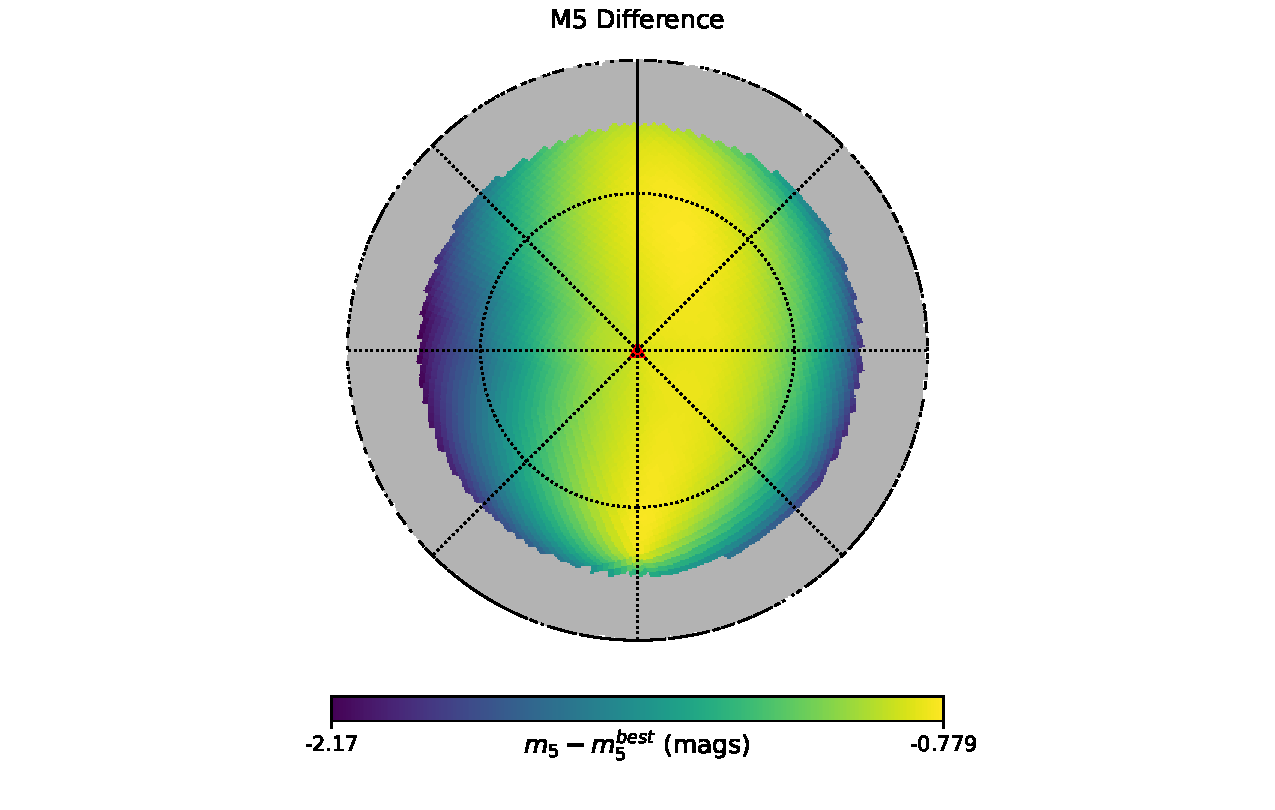
\includegraphics[width=0.4\textwidth]{figs/m5diff.pdf}
  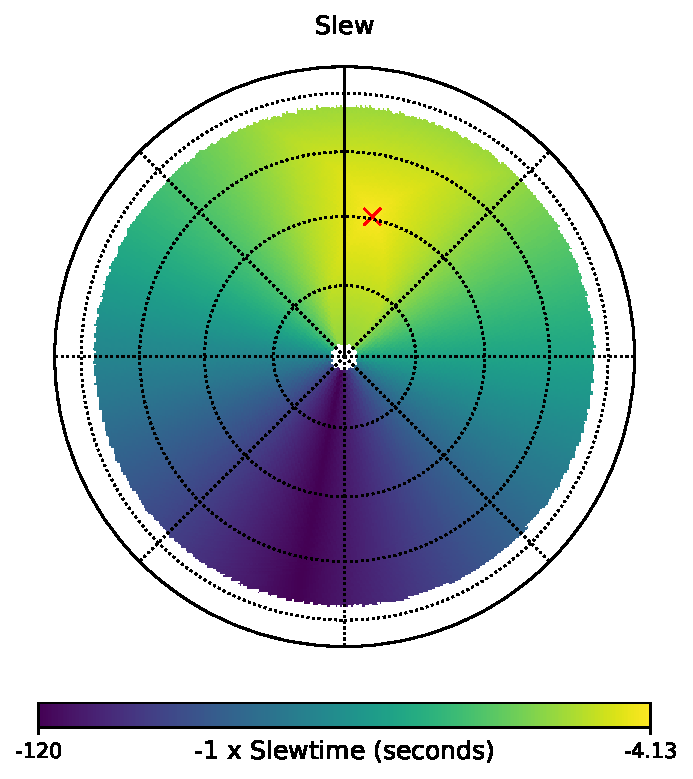
\includegraphics[width=0.4\textwidth]{figs/slew.pdf}
  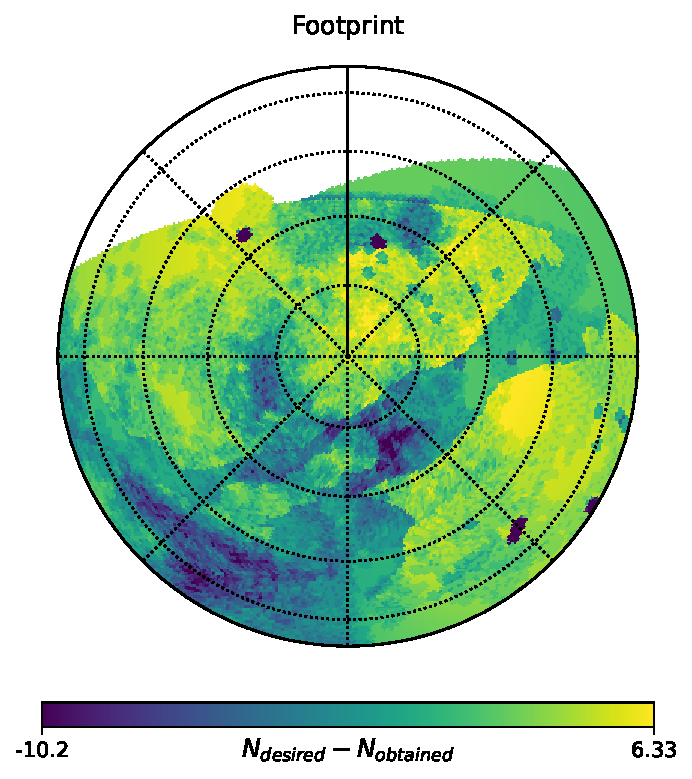
\includegraphics[width=0.4\textwidth]{figs/footprint.pdf}
  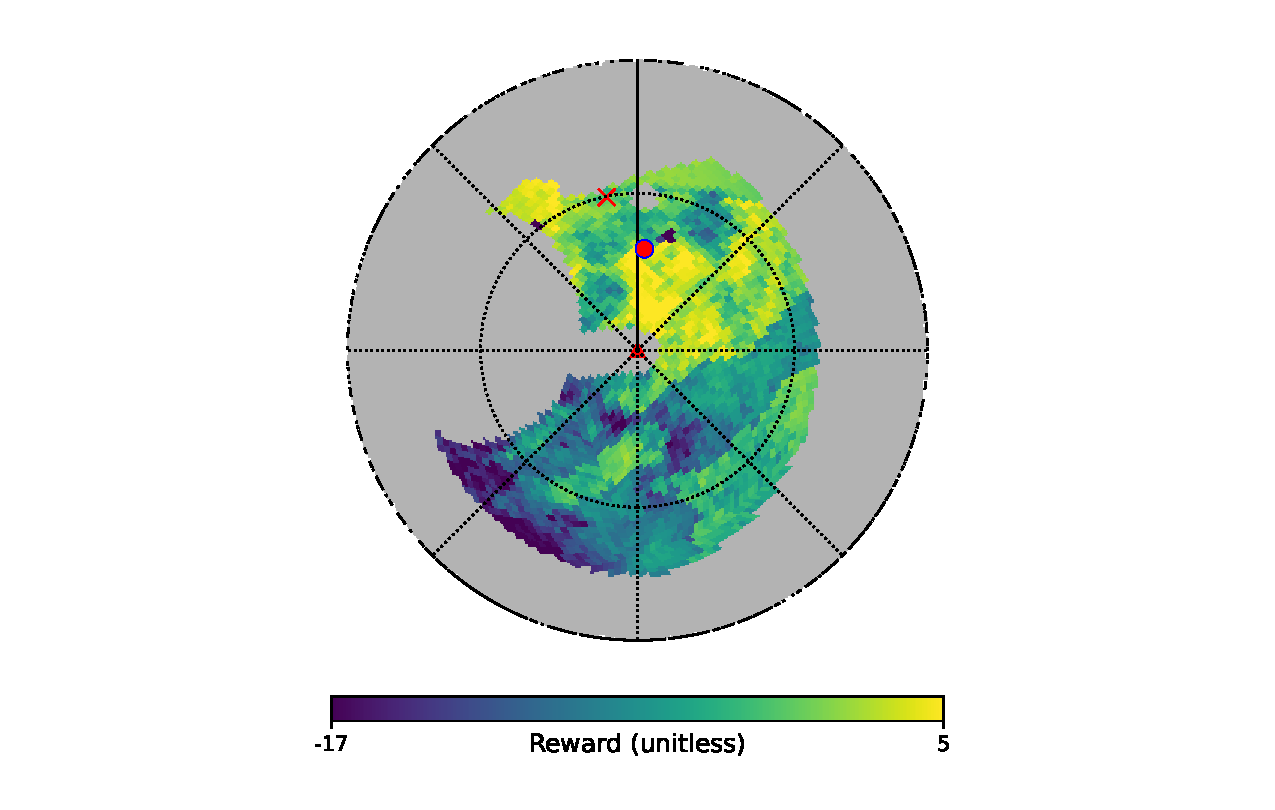
\includegraphics[width=0.4\textwidth]{figs/survey_choice.pdf}
  \caption{The primary basis functions to balance image depth, uniform coverage, and on-sky efficiency
  are the M5DiffBasisFuntion, the SlewBasisFunction, and the FootprintBasisFunction, shown in the first three 
  panels respectively.  The red triangle indicates the location of zenith, above Rubin, and in the SlewBasisFunction,
  the red X marks the current pointing of the telescope. These, combined with additional basis functions to fine tune
  survey visit choices and including the standard masks from Figure~\ref{fig:masks}, are shown in the final panel.
  The final panel also shows the next pointing that would be chosen by this survey, as a red circle. }
  \label{fig:rewards}
\end{figure}

\paragraph{FieldSurvey.}
The \texttt{FieldSurvey} is intended for use with a single chosen pointing and
can execute a predefined sequence of observations each time it is selected, while
still using basis functions to prioritize one \texttt{FieldSurvey} against
another. A simple example is a \texttt{BasisFunction} that enforces a minimum
revisit gap after the last visit to a given field before the survey can be chosen
again, combined with a slew-time basis function that encourages shorter slews. If
multiple \texttt{FieldSurvey} instances are configured with these basis
functions, the FBS cycles through the fields at an interval equal to or longer
than the revisit gap, obtaining the predefined observation sequence at each
field's location and moving to the next nearest field after each sequence.

\subsection{Masks and Constraints}
\label{sec:masks}

All \texttt{Survey} classes can accept \texttt{BasisFunction} instances that act
as masks, removing inaccessible areas of sky or restricting available observation
choices as necessary. This mechanism ensures that all surveys obey the same
constraints and that the observatory operates safely within limits. The standard
masks applied to all surveys include:
%
\begin{itemize}
  \item Altitude and azimuth limits, including a zenith exclusion zone where
    tracking for the Simonyi Alt/Az mount is difficult.
  \item A Moon avoidance mask that ensures the telescope points no closer than
    30\,degrees from the Moon, protecting the LSSTCam.
  \item A planet avoidance mask that excludes Jupiter, Mars, and Venus, as these
    bright planets move quickly enough that it is preferable to avoid them rather
    than attempt to observe through them.
\end{itemize}

Figure~\ref{fig:masks} illustrates these standard masks at a specific time

During commissioning, an additional mask ensured that the Simonyi telescope
remained pointed away from the rising Sun during the last three hours of the
night, in case dome closure was delayed by system issues.

\begin{figure}
  \centering
  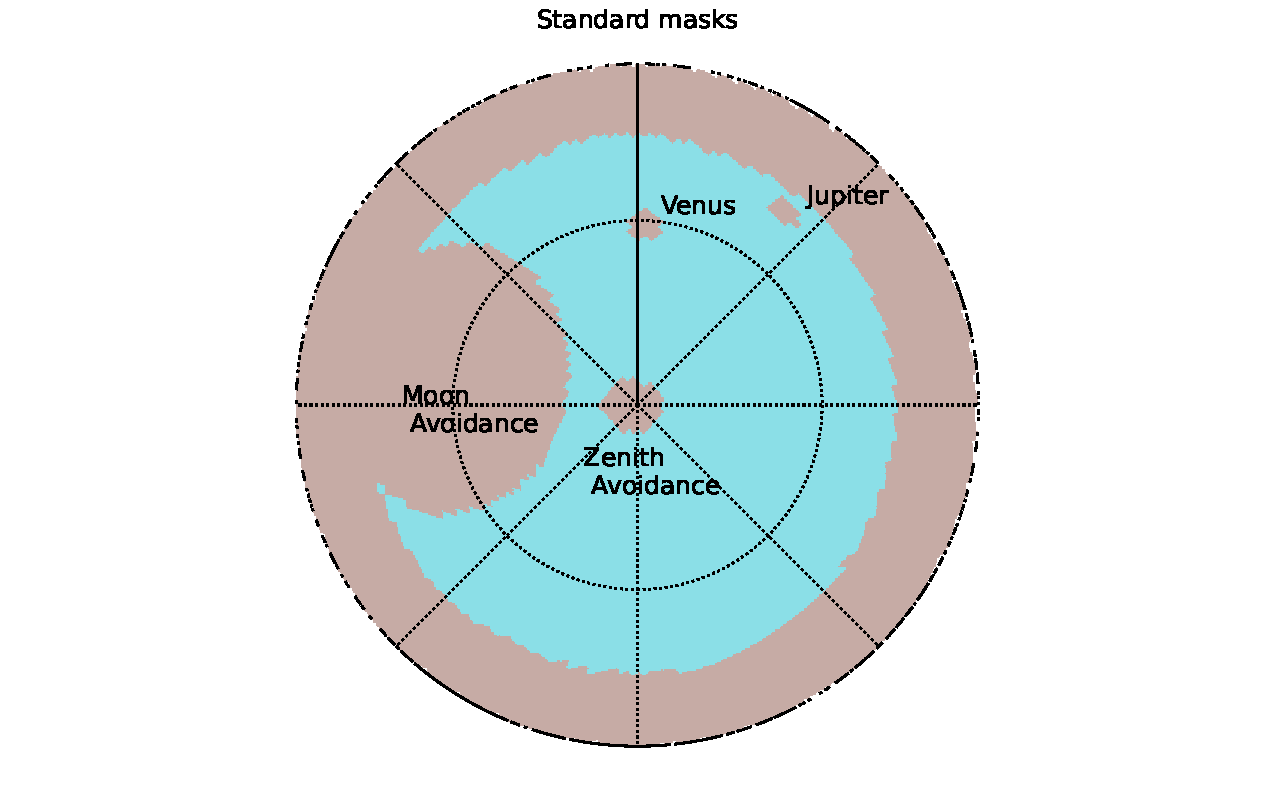
\includegraphics[width=0.8\textwidth]{figs/standard_masks.pdf}
  \caption{Example sky map showing the standard masks applied to all
    \texttt{Survey} classes. Masked regions above the horizon are shown in brown and include
    altitude and azimuth limits (with a zenith exclusion zone), a
    30\,degree Moon avoidance zone, and exclusion regions around Jupiter
     and Venus (Mars is not visible).  The
    unmasked area (light blue) represents the sky available for scheduling at
    this example epoch. The red triangle indicates the location of zenith, above Rubin.}
  \label{fig:masks}
\end{figure}



\subsection{Operational Cycle}
\label{sec:operational_cycle}

The FBS operates in a continuous cycle of three steps:
%
\begin{enumerate}
  \item \textbf{Update telemetry} ---
    \texttt{CoreScheduler.update\_conditions()} ingests the current observatory
    and environmental state.
  \item \textbf{Request observation} ---
    \texttt{CoreScheduler.request\_observation()} evaluates all configured
    surveys and returns the highest-priority feasible observation.
  \item \textbf{Record observation} ---
    \texttt{CoreScheduler.add\_observation()} feeds the completed observation
    back into the scheduler, updating internal state.
\end{enumerate}
%
This cycle repeats continuously while the FBS is in operation.


\section{Survey Simulations}
\label{sec:simulations}

The algorithms in the FBS are designed to make pointing decisions throughout the
night under realistic observing conditions, while working towards scientific goals
that can only be realized after much longer timeframes. To tune these algorithms and select
the overall survey strategy that best satisfies the wide range of LSST science
goals at the end of the ten year survey, the FBS is often run in a simulation mode using the same
\texttt{rubin\_scheduler} code base as in real-time operations---with simulated
telemetry replacing measurements from the summit and a model of the
observatory's response replacing actually acquired observations.  
This allows us to test variations on the scheduler configuration as well as generate 
predictions for survey performance into the future.

The FBS has been tested and developed against simulated telemetry and
observation models since 2018, beginning with the LSST Call for White Papers on
cadence optimization~\cite{PSTN-001}. Over 1000 simulated surveys
have been produced to date, refining the scheduler configuration to balance science performance
under the guidance of the Survey Cadence Optimization Committee (SCOC). 
The process of optimizing the survey strategy is
documented in Bianco et al.~\cite{2022ApJS..258....1B} and has involved significant
input from the broader astronomical community. Simulations will continue
throughout operations, responding to evolution in the scientific landscape and
providing a means to evaluate the impact of observatory performance updates.

\subsection{Sky and Atmospheric Models}
\label{sec:env_models}

To support survey strategy simulations, we have developed high-fidelity models
of the expected sky conditions. An atmospheric seeing database based on
historical DIMM measurements from CTIO~\cite{RTN-XXX} is combined with the
expected system contribution to seeing to produce wavelength- and
airmass-dependent estimates of delivered image quality. A model of sky
brightness as a function of time, bandpass, and position on the sky has been
validated against on-site measurements at the summit~\cite{SKYBRIGHT}.
Combining these models with the expected optical throughput of the telescope
yields an estimate of the five-sigma point-source depth for each image. Weather
downtime is extrapolated from historical cloud-coverage records collected
on-site~\cite{WEATHER}.

\subsection{Observatory Performance Models}
\label{sec:obs_models}

The model of observatory performance includes a high-fidelity model of the
telescope itself, used to evaluate the slew time required between pointings.
Estimates of scheduled downtime due to planned engineering and maintenance, as
well as unplanned downtime due to faults or technical issues, are also
incorporated.


\section{Early On-sky Use}
\label{sec:onsky}

At the summit, the FBS operates within the observatory's Scheduler Commandable
SAL Component (SchedulerCSC). The SchedulerCSC manages all interfaces with the
observatory itself---gathering telemetry, commanding pointing requests, and
handling the timing and queuing of observations selected by the FBS.

\subsection{Auxiliary Telescope}
\label{sec:auxtel}

Initial on-sky use of the FBS began with the Auxiliary Telescope (AuxTel) in
early 2022. This early deployment exercised the end-to-end integration of the
FBS into the SchedulerCSC: gathering telemetry, passing it to the FBS, receiving
requested pointings, commanding the telescope, and reporting acquired
observations back to the FBS. It also provided preliminary testing of the methods
used to track how the FBS was configured and run and what artifacts were
preserved to support identification of unanticipated scheduling choices.

However, AuxTel operation differed from the eventual LSST use case in several
important respects. AuxTel's data-acquisition rate was much lower and its
instrumentation more varied---it was frequently operated with a spectrograph
rather than an imager alone---so the cycle of requesting and reporting
observations was considerably simpler. The slower cadence and longer exposures
also gave observing specialists more opportunity---and more need---to modify
observations as they were acquired (e.g., changing the order or repeating a
failed observation), and these ad hoc variations were difficult to capture
in the recorded artifacts. The scheduling decisions themselves were also
simpler: the target list was short and the selection algorithms bore little
resemblance to those required for the full LSST survey. AuxTel use was therefore
extremely valuable for integration testing but was not expected to be sufficient
to fully commission the FBS for LSST survey-style observations.

\subsection{Simonyi Telescope Commissioning}
\label{sec:simonyi_onsky}

At the start of on-sky commissioning with LSSTCam on the Simonyi telescope, the
FBS was used to execute simple observing programs consisting of a small number of
fields observed through a fixed sequence of bandpasses. Similar programs had
previously been carried out with LSSTComCam. These tests served as further
integration exercises for the FBS and SchedulerCSC on the Simonyi telescope, but
the programs themselves were deliberately simple: telemetry requirements were
minimal, and observations for a given field were effectively triggered by the
observing specialist pointing the telescope to the chosen field and then enabling
the corresponding FBS configuration. This configuration, like the earlier AuxTel configurations,
included only a collection of \texttt{FieldSurvey} instances, configured to acquire sequences
of individual fields with the choice of field driven primarily by the Observing Specialists
by including only a SlewBasisFunction. 

The full Science Validation (SV) survey with LSSTCam began at the end of April
2025, marking the first deployment of an FBS configuration comparable in
complexity to the full LSST survey. The SV survey plan is described in
\cite{SITCOMTN-005}; in brief, approximately 3{,}000\,deg$^{2}$ along the
ecliptic were targeted for observations in a mode roughly approximating standard
LSST Wide-Fast-Deep operations, albeit with a denser cadence and a smaller
overall footprint. Planning for the SV survey was itself supported by simulations
run with the FBS, which were used to position the 3{,}000\,deg$^{2}$ footprint
on the sky for optimal visibility during the SV observing period.

\subsubsection{Debugging with Artifacts}
\label{sec:debugging}

Debugging situations where the FBS did not behave as expected is supported
by artifacts saved by the
SchedulerCSC during operations. These artifacts include a
snapshot of the telemetry (\texttt{Conditions}) passed to the FBS and a
serialized copy of the FBS itself after ingesting that telemetry. Together, these
snapshots allow us to recreate the FBS at the exact moment observations were
requested and inspect its full internal state to understand why particular
observations were chosen. Additional records include the list of upcoming
requested observations (``targets'') and completed observations
(``observations''), both recorded in the LSST Engineering Facilities Database
(EFD). A few examples of issues found and resolved during this phase
include:
%
\begin{itemize}
  \item \textbf{Unexpected slew to an unrelated field.}
    After an initial image series, the FBS unexpectedly slewed away from the
    intended field. The targets, observations, and telemetry all appeared
    reasonable, but recreating the FBS from its snapshot reproduced the runaway
    behavior. The root cause was a configuration error: the field selection was
    driven by a slew-time basis function that was configured per-bandpass, and the
    final bandpass in the observation sequence had been omitted from that
    configuration by oversight. The FBS configuration was updated accordingly.

  \item \textbf{Incomplete bandpass sequence.}
    The FBS requested observations in several bandpasses, but only two were
    acquired. The FBS snapshot confirmed that the full sequence had been
    requested, yet the recorded targets contained only a subset. The issue was
    traced to a parameter in the SchedulerCSC that limited the maximum rate of
    filter changes for engineering reasons; this limit needed to be increased
    to permit the intended program to execute.

  \item \textbf{Dropped observations in a dither pattern.}
    A requested dither sequence was only partially acquired. The FBS snapshot
    again confirmed that the complete set of observations had been requested, but
    some did not appear in the recorded targets. Correlated records in the EFD
    revealed that observing-script failures immediately prior to the missing
    observations had caused them to be dropped, requiring adjustments in the
    SchedulerCSC's handling of script failures.
\end{itemize}

Investigating these issues also led to improvements in the artifact-recording
process itself. In particular, the cadence of FBS snapshots was increased from
every other observation request to every request. The lower cadence had been
adequate for AuxTel's single-observation-at-a-time mode but was insufficient
for the longer observation sequences used on the Simonyi telescope. Overall,
the artifacts recorded by the FBS and SchedulerCSC have proven invaluable and
have been sufficient to diagnose the majority of issues encountered to date.



\subsection{Pre-night Simulations vs.\ On-sky Outcomes}
\label{sec:prenight}

% TODO: compare pre-night FBS simulations with the observations actually
% acquired during commissioning and early operations.

\section{Lessons Learned}\label{sec:lessonslearned}

configuration challenges and process

downstream data management needs

interactions with the SCOC and the community

\section{Conclusions}\label{sec:conclusions}

Working well, evolving simulations.

